\section{Ejercicio 01}\label{sec:ejercicio1}

\begin{frame}{Oscilador Amortiguado}
    \begin{itemize}
            \item Masa de la partícula - $m = 70\ kg$
            \item Tiempo de simulación - $tf = 5\ s$
            \item Constante elástica - $k = 10000\ kg/s^2$
            \item Viscosidad - $gamma = 100\ kg/s$
            \item Amplitud inicial - $A = 1\ m$
        \end{itemize}
    \text{Animation :D https://youtu.be/X2C-ouZ1_7g}
\end{frame}

\begin{frame}{Oscilador Amortiguado}
    \begin{figure}[H]
        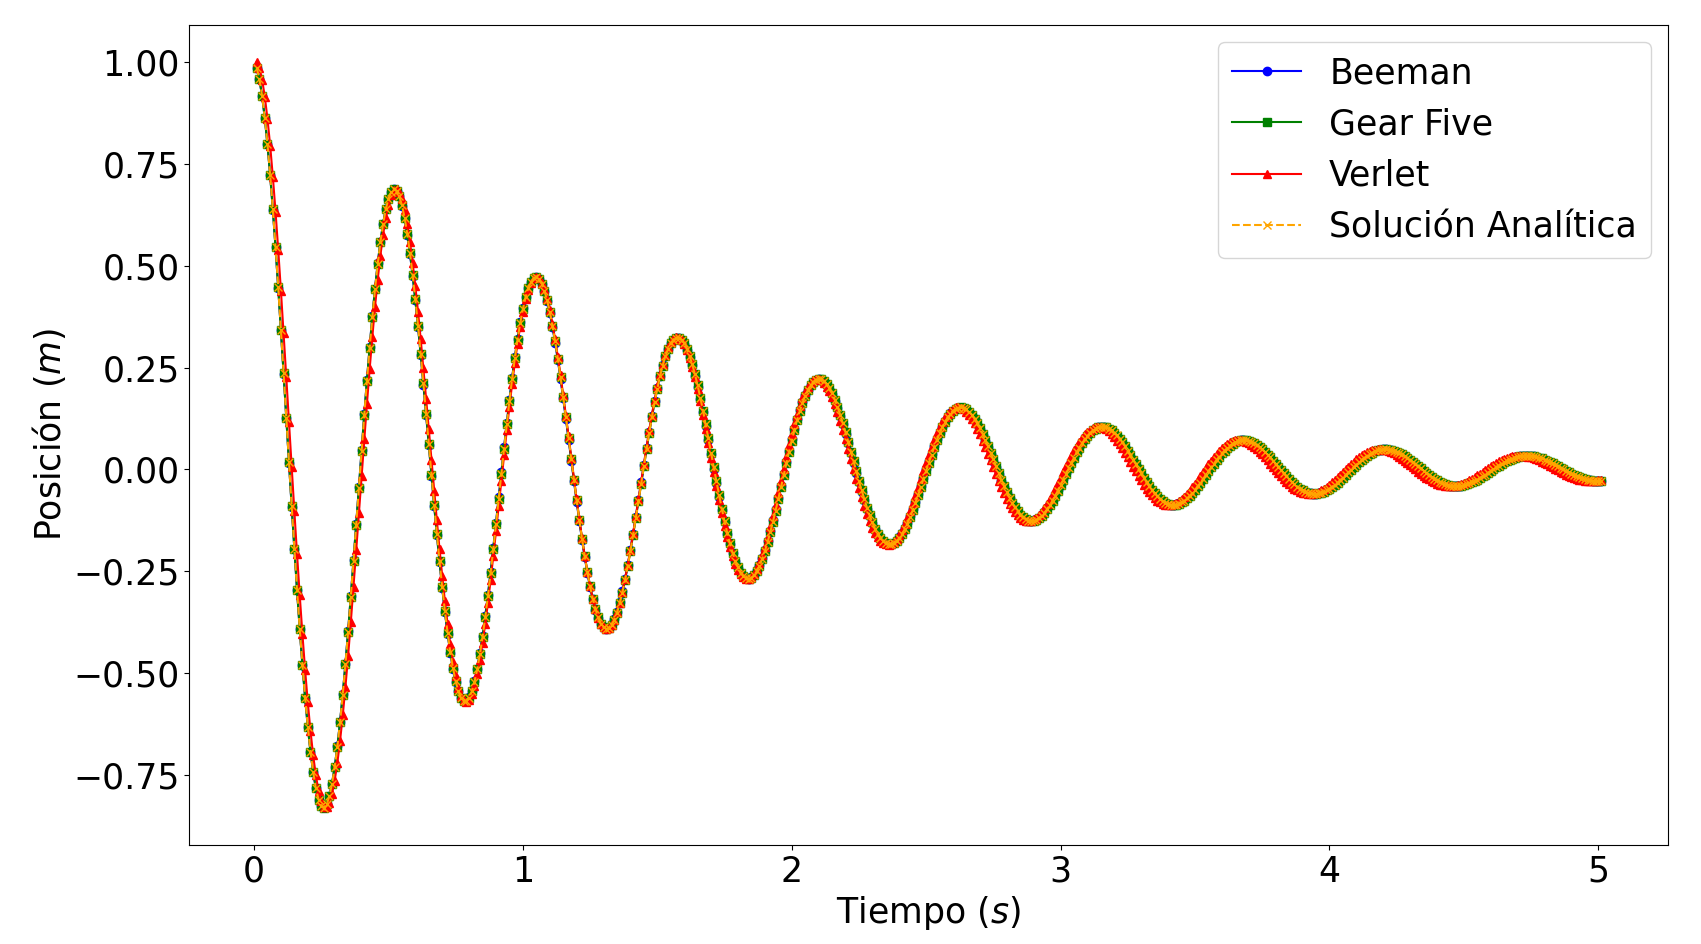
\includegraphics[width=1\linewidth]{pic/00-ejercicio1/todos.png}\label{fig:osciladores}
        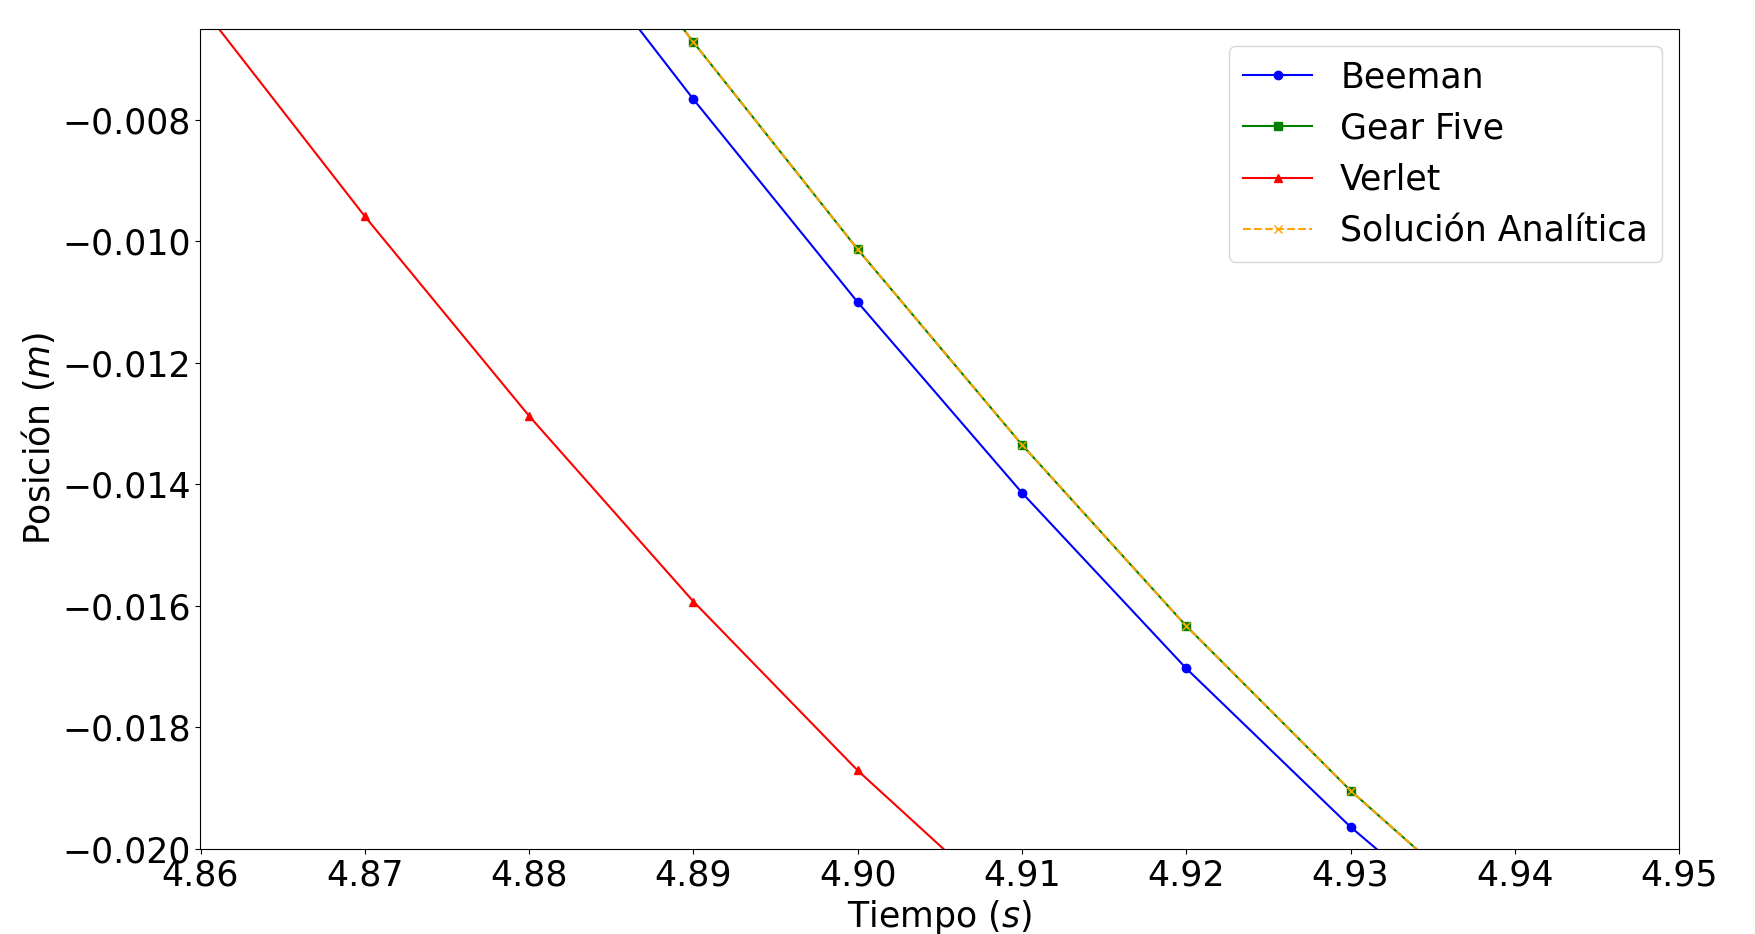
\includegraphics[width=1\linewidth]{pic/00-ejercicio1/zoom.png}\label{fig:osciladoreszoom}
    \end{figure}
\end{frame}

\begin{frame}{Oscilador Amortiguado}
    \begin{figure}[H]
        \centering
        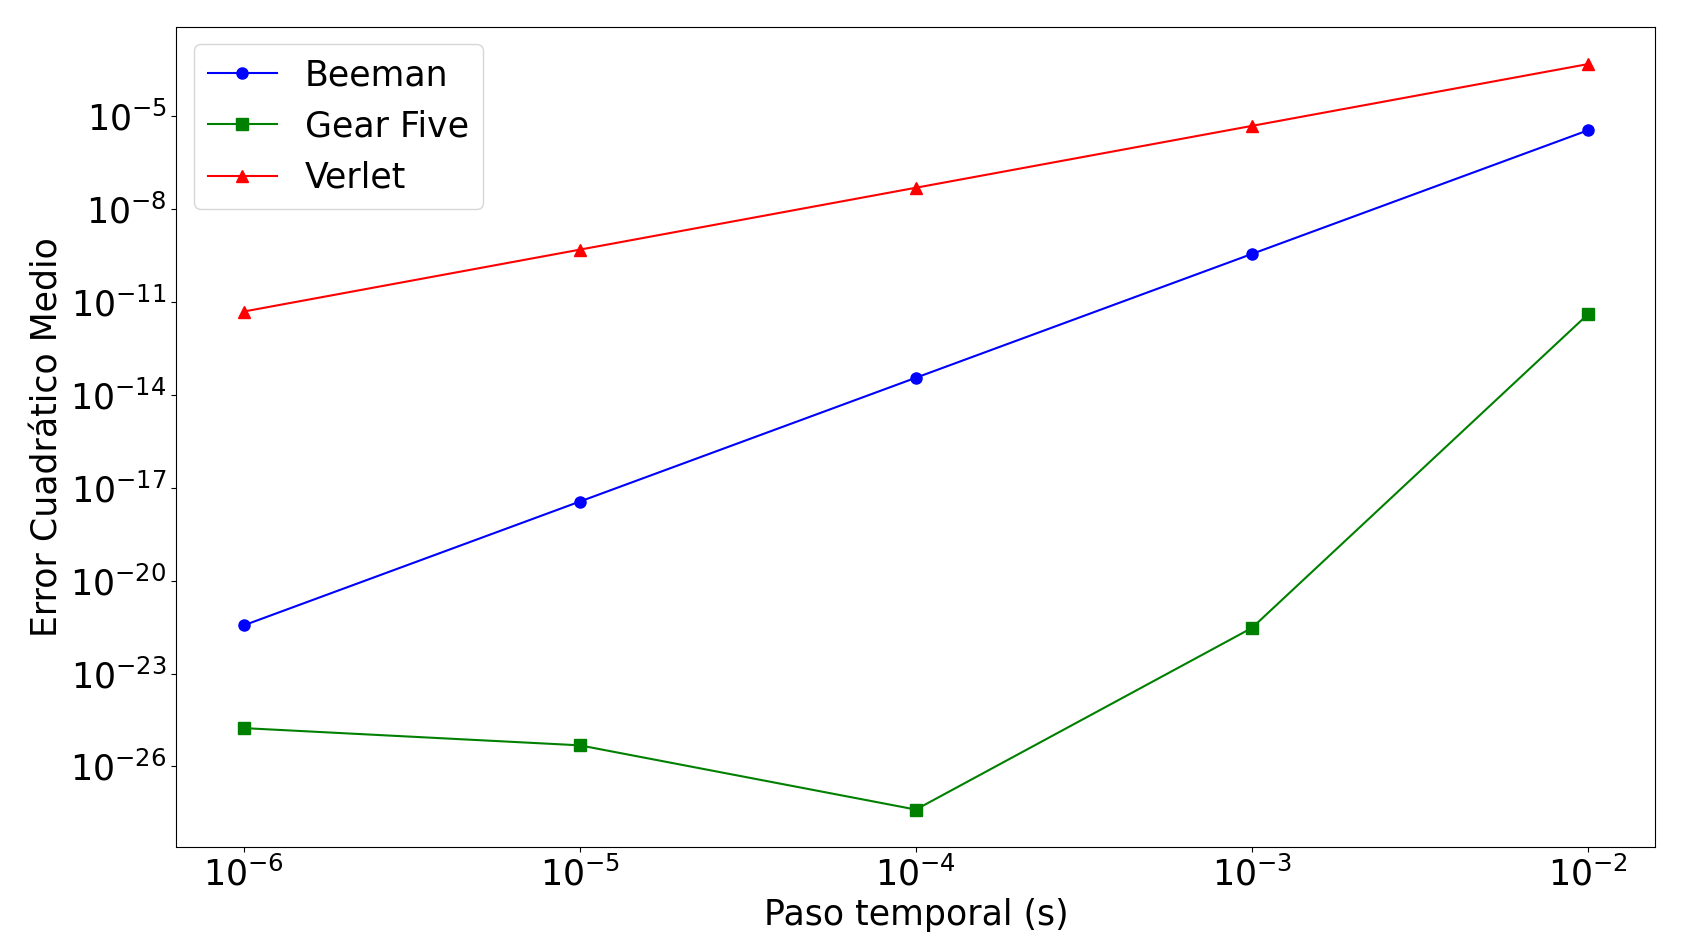
\includegraphics[width=1\linewidth]{pic/00-ejercicio1/ECMs.png}\label{fig:osciladore-ECM}
    \end{figure}
\end{frame}
